\section{Design}
In this section, the design of the different parts of the system, and their interactions, are presented.


\subsection{Back end}
\label{sec:back-end}
The diagram shown on \ref{fig:serversidestructure} describes the overall structure of the server-side of the system. The server-side consists of both the Web-service, accessed through an API, and the control panel. These has been combined since they both interact with the same database and both use the same model. 

\begin{figure}[H]
    \centering
    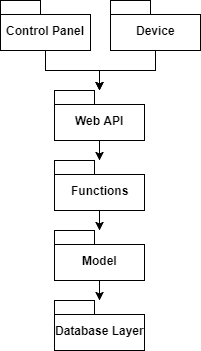
\includegraphics[width=0.4\textwidth]{Figures/serverSide.png}
    \caption{The structure of the server-side part of the system}
    \label{fig:serversidestructure}
\end{figure}

The function-layer is split into two parts, one for the control-panel and one for the API. This is done to isolate the functionality, such that each component only has access to their needed functionality. The shared model layer can be seen on figure \ref{fig:serversidemodel}.

\begin{figure}[H]
    \centering 
    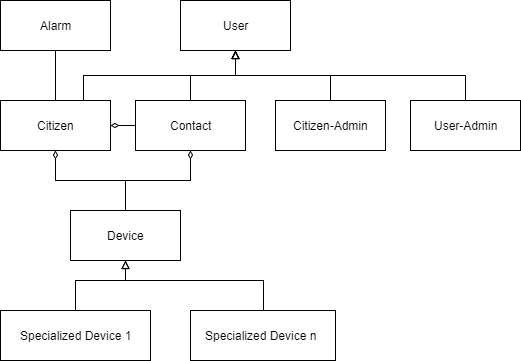
\includegraphics[width=0.9\textwidth]{Figures/serverSidemodel.png}
    \caption{The back end model-layer}
    \label{fig:serversidemodel}
\end{figure}

There is eight classes in the model, each representing different aspects of the system. There is a super class \textit{User}, which represents a user in the system. Each user type, inherits from this super class. The different user types represented in the system are: \textit{Citizen}, \textit{Contact}, \textit{Citizen Admin} and \textit{User admin}. Besides the user-related classes, there is also a \textit{Device} and \textit{Alarm} class. Each of these different classes, found on the class-diagram, and their relationship, is described in details in this section.

\paragraph{User} is the super class used for all user types in the system. It contains, among others, the required login information to access the system.

\paragraph{Citizen} inherits from User. It represents a citizen in the system, and has references to contacts and devices. 

\paragraph{Contact}

\paragraph{Citizen Admin}

\paragraph{User Admin}

\paragraph{Device} represents a device in the system, either used by the citizen or contact.

\paragraph{Alarm} contains information about an active alarm. It contains information about who triggered the alarm, the current status of the alarm


\subsection{Web-Service}
When designing a web-API for a service, it is important to consider which architecture to use and how to facilitate the communication to and from the service. Considering the requirements given in section \ref{sec:non-requirements}, the architecture must allow for easy communication between devices.

There are different ways to communicate with a web service, where the most noticeable are REST, WSDL, and SOAP. WSDL and SOAP are standards for how communication between a client and server should happen, while REST is an architecture, but a standard by itself.
Both WSDL and SOAP are structured as objects in XML that are then sent to the server. REST uses the HTML protocol, and have no fixed format that has to be followed. That makes REST easier and more flexible to work with. Most modern tools are also build with REST as the focus of the three, so we will continue working with REST, which we describe below in subsection \ref{rest}.

%we need a way to interact with it. Here we will look at different ways to interact with a server or service through the use of a Web-API.

\subsection{REST} \label{rest}
\todo{source pdf}
REST is based on the HTTP protocol, and a REST system allows a client to communicate by using HTTP messages \cite{restapitutorial}\cite{restwikipedia}.
The four common message types used in REST are:

\paragraph{GET} gets a representation of a resource. The use of GET should never have side effects, and multiple calls to get should always give the same result.
\paragraph{DELETE} deletes a resource. Trying to delete a resource that doesn't exist usually results in an error response, such as 404. DELETE is also idempotent, so sending it multiple times does not cause any damage to the rest of the system, should it be sent twice.
\paragraph{POST} creates a new resource. Unlike DELETE, POST is not idempotent, so sending the same request twice will create the resource twice. 
The standard also allows POST to be overloaded. POST can do any change: DELETE, PUT, PATCH. When overloading POST, there are no protocol semantics it has to follow.
\paragraph{PUT} updates an existing resource. PUT is also idempotent, as sending the same PUT message multiple times will just update the resource to what it already is. Put can also work as POST for when the resource does not exist.

\subsubsection{Rest constrains}
REST has six constrains that has to be fulfilled for a Web-API to be RESTful, these are as follows.

\paragraph{Uniform Interface}  There are four principles for a uniform interface:
\begin{itemize}
\item REST is resource based, so all data is sent between server and client using URIs.
\item When a client has a resource, it should also have enough data to modify it and send the modified resource back to the server.
\item Each message should be self-descriptive, meaning the message itself should contain information about how it should be read.
\item Clients deliver state by using hypermedia (body contents, query-string parameters, request headers and request URI).
\end{itemize}

\paragraph{Stateless} A REST implementation is stateless if the server has no knowledge of the state of the client. All relevant data for the state of the client has to be sent to the server at each call, and nothing is kept between calls.

\paragraph{Cacheable} Some responses can be cached, while others cannot. So a resource must know if it can become stale between uses.

\paragraph{Client-Server} Clients should not be concerned with storage of data, while the server should not be concerned with user interface or user state. As long as the interface between server and client is unaltered, they can be developed independently.

\paragraph{Layered System} A client cannot tell if it is talking to the endpoint, or an intermediary. This allows load-balancing as multiple intermediary servers can run on multiple physical units, and still connect to the same end-point.

\paragraph{Code on Demand} The server can extend its functionality by sending logic that can be executed by the client. This step is unlike the others optional for an API to be RESTful.


\subsection{Control panel}
The diagram shown on \ref{fig:controlpanel} describes the different views in the control panel. 

\begin{figure}[H]
    \centering
    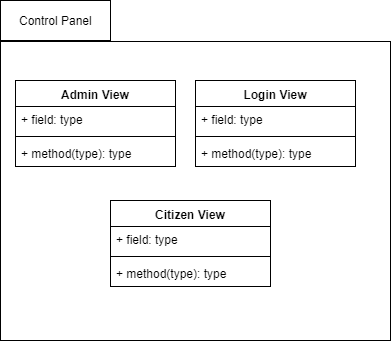
\includegraphics[width=0.4\textwidth]{Figures/ControlPanel.png}
    \caption{The different views included in the control-panel}
    \label{fig:controlpanel}
\end{figure}

The login view is the first view shown, when a user accesses the cite. This view allows them to login to the system and gives access the rest of the views.

The admin view, is the view shown to users with administration rights. The view will make the admin able to add new users or edit existing users to the system from the view.

The citizen view is for users with citizen-admin rights. The view will show the information on all the citizen the citizen-admin is administrating and allow them to add to these or edit the existing.

\subsection{Smartphone app}
The smartphone app is one of the components where interaction with the citizens takes place. It is designed as an app and an underlying fall-detection service, which then interacts with the web-service, using the web-API.


\begin{figure}[H]
    \centering
    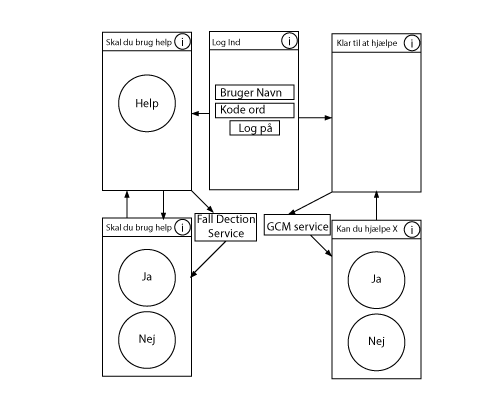
\includegraphics[width=1.0\textwidth]{Figures/MobilUI.png}
    \caption{Prototype of smartphone UI}
    \label{fig:mobilUI}
\end{figure}

Figure \ref{fig:mobilUI} shows an early low fidelity prototype of the app. It illustrates both the flow though the views and their individual designs, the views are numbered 1 to 5 in red this is not part of the app, but has been added to make it easier to refrence each view.

%\todo{we need names on the diagram of the different views, or numbering of it}

View 1 (\textit{log-in-view}) is the first view that the user meets. Here the user needs to log in, and the app then change to either View 2 (\textit{citizen-view}) or View 4 (\textit{contact-view}), depending on the type of user that is returned from the web-service when logging in.

The \textit{citizen-view} consists of a button to call for help, which when clicked will then change to a \textit{confirm-help-view}. In the view 3 (\textit{confirm-help-view}) the citizen has to confirm that they need help or dismiss it (either verbally or by physically clicking the button). If not input is given the view will time out and call for help. This view is also shown when the apps fall-detection service detects a fall. The fall-detection service is running even when the main app is not.

The \textit{contact-view}, is reached when logging in as a contact. A contact will only leave this view when they receive an alarm from an associated citizen. This alarm will come in the form of notifications. When the contact reacts to the notification, they will open \textit{view 5} where the name of the citizen in need of help, is shown. The contact must then either confirm that they can and will help the citizen or reject the call for help. The app then sends this response to the web-service.

\subsection{Personal assistant}
To be able to design the personal assistant, it is important to understand the platform and its limitations. For this reason, this section starts by exploring some different platforms, and picking one suited for this project. \todo{Færdiggør mig}


\subsection{Communication}
In this section process diagrams are presented to better understand how the different devices communicate with and through the Web-Service, using the API. These are different from the diagrams found in section \ref{sec:system-behaviour}, since these shows how the different components communicate, where as the ones described earlier shows how the different actors (with the system being one) interacts with each other. 

Each diagram describes the communication during a specific event. 

It can be seen on figure \ref{fig:post-alarm} how a citizens device posts an alarm to the Web-Service.

\begin{figure}[H]
    \centering
    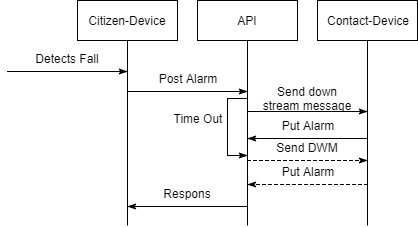
\includegraphics[width=0.7\textwidth]{Figures/Citizen_to_Contact.png}
    \caption{Communication between devices during an alarm activation}
    \label{fig:post-alarm}
\end{figure}

When a citizen device detects a fall, this process is described in section \ref{sec:system-behaviour}, it posts an \textit{Alarm} to the web-API and waits for a response. When the API receives an alarm, it immediately sends a message to the contact person associated to the citizen, with the highest priority and starts a timer. If the web-service does not receive an answer from the device and the timer runs our, or it receives a rejected alarm from the contact, then the system sends the same alarm to the next contact person on the list. This is repeated until, either a contact responds with an accepted \textit{Alarm} or there is no more contacts on the list. When the API receives an accepted alarm or runs out of contacts, it sends a response to the citizen-device with information regarding who, if any, has responded.\todo{Måske skal den ikke bare slutte}

\begin{figure}[H]
    \centering
    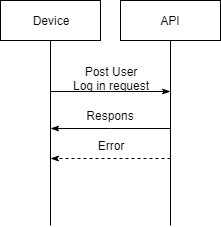
\includegraphics[width=0.4\textwidth]{Figures/Device-Api.png}
    \caption{Communication between devices during sign-in}
    \label{fig:post-sign-in}
\end{figure}

During a \textit{login} event, the system reacts as seen on figure \ref{fig:post-sign-in}. If the request is successful, the service will return the corresponding user, if not, it returns an error.

\subsection{Database design} \label{sec:databasedesign}
To get a better understanding of the design of the database, used in this project, an ER diagram is shown on figure \ref{fig:database}.

\begin{figure}[H]
    \centering
    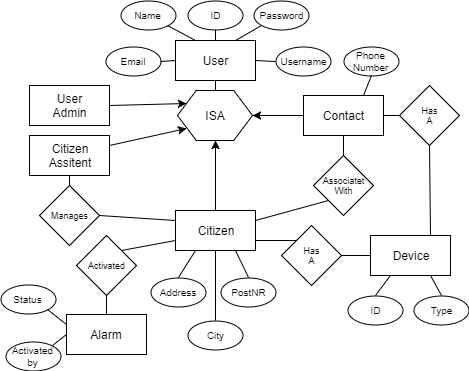
\includegraphics[width=1.0\textwidth]{Figures/Database.png}
    \caption{Database design}
    \label{fig:database}
\end{figure} \todo{Diagrammet vil komme til at ændre sig da der er et par ændringer vi er nødt til at lave i databasen.}

The database design consists of seven entities, where four of these are specifications of the \textit{User} entity. These specifications are \textit{Citizen}, \textit{Contact}, \textit{Citizen admin} and \textit{User admin}, and represents the different user types that can exist in the system, as described in section \ref{sec:back-end}. 

The last two entities are \textit{Alarm} and \textit{Device}. The \textit{Alarm} entity represents an alarm in the system, it has a foreign key \textit{Activated by} that points to the citizen who has activated the alarm and a status property that represents the current state of the alarm. The \textit{Device} entity represents the devices that citizens and contacts has.